\section{Proposed Architecture} \label{arch}

\subsection{Overview}

The TorCoin architecture implements the novel TorCoin and TorPath protocols. We
describe both in later sections, but in brief, the TorCoin protocol mines
coins, and the TorPath protocol assigns a circuit (entry, middle, and exit
servers) to each client.

TorCoin runs as a standalone service, and requires very little modification of
the core Tor codebase. Tor clients and relays operate as usual, but receive
circuit assignments from \textit{assignment servers} instead of directory 
servers. Separately, a \textit{TorCoin Miner} on each machine mines TorCoins
by monitoring the throughput of the local Tor TLS tunnel, and communicating with its circuit neighbors via the TorCoin algorithm.

Figure \ref{figure:archi} shows a basic overview of this architecture.

\begin{figure}
  \centering
    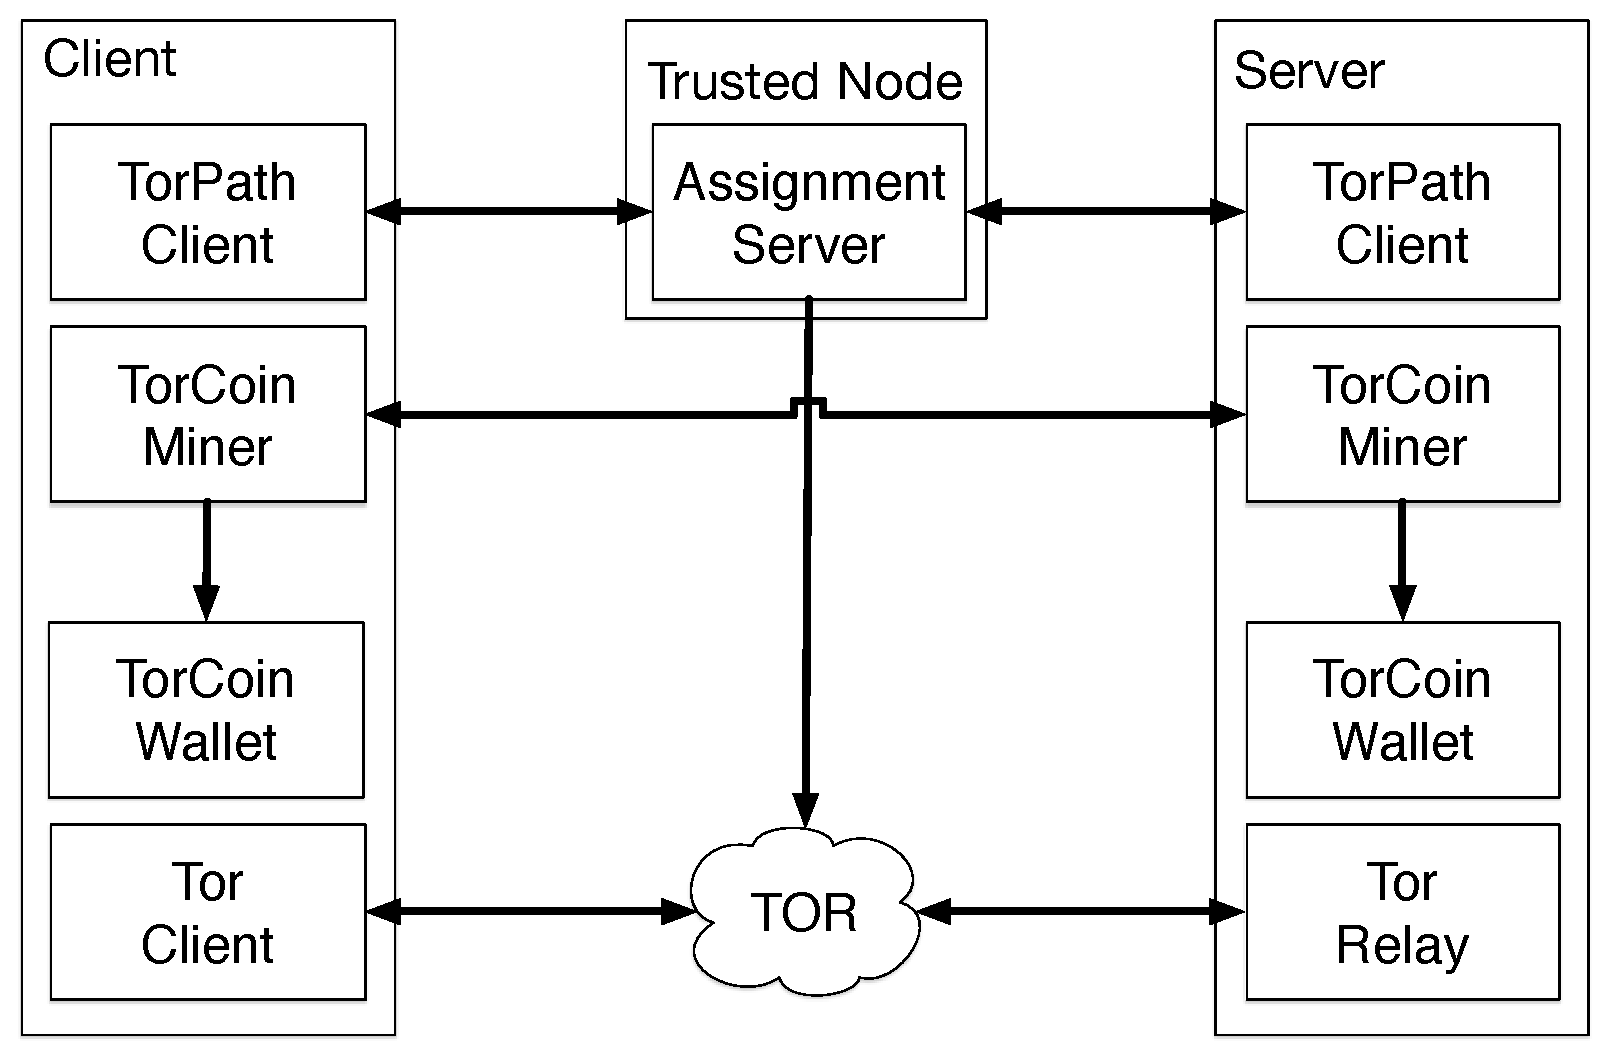
\includegraphics[scale=0.3]{architecture.pdf}
  \caption{High level TorCoin system architecture for clients and relays. A \textit{TorPath Client} assigns Tor circuits to clients via the TorPath protocol, described in the next section. A \textit{TorCoin Miner} mines TorCoins and stores them in a \textit{TorCoin Wallet}. Each \textit{Tor Client} and \textit{Tor Relay} operates as usual, but on circuits assigned via the TorPath protocol.}
  \label{figure:archi}
\end{figure}


% TorPath is an anonymous cooperative routing protocol that randomly assigns
% circuits to Tor clients using decentralized, cryptographically verifiable
% methods. It consists of groups of assignment servers, which are ``trusted'' in
% the same way as Tor directory servers, and a TorPath client to communicate
% with them.  Groups of assignment servers use the distributed TorPath protocol
% to  keep track of available relays and assign circuits to clients.

% The TorCoin algorithm is used to reward nodes for transferring bandwidth. It
% consists  of a TorCoin miner and a TorCoin Wallet. The TorCoin miner measures
% Tor bandwidth by monitoring the  throughput of the local Tor TLS tunnel,
% allowing us to avoid modifying internal  Tor code. It also sends out TorCoin
% packets that serve as ``proof-of-bandwidth''. The TorCoin Wallet is a
% cryptographic wallet for storage of coins and transactions. When the miner
% discovers a new TorCoin, it adds it to the blockchain with all the information
% necessary for anyone to verify it.


\subsection{Adversary Model} We consider the existence of an adversary who
wishes to obtain TorCoins without trnsferring bandwidth. We assume the
adversary is able to control a number of clients and routers. We assume that
malicious clients and routers know about each other's existence and are able
to collude. We also assume that the adversary is able to control a minority of
Assignment Servers on the network.

% Original text:
% \subsection{TorPath Components} TorPath is an anonymous cooperative routing
% scheme that randomly assigns circuits to Tor clients using decentralized,
% cryptographically verifiable methods. It requires groups of assignment servers,
% which are ``trusted'' in the same way as Tor directory servers, and a TorPath
% client to communicate with them. 

% \subsubsection{Assignment Server} A small set of trusted nodes run the
% Assignment Servers, which perform similar roles to the current Tor directory 
% servers. Groups of assignment servers use the distributed TorPath protocol to 
% keep track of available relays and assign circuits to clients.

% \subsubsection{TorPath Software} Clients and relays install the TorPath Software to
% communicate with Assignment Servers, using the TorPath protocol to retrieve
% circuits (clients). 
% % To avoid modifying Tor client code, TorPath can use a local 
% % DNS proxy to redirect requests to directory servers to the new assignment servers.

% \subsection{TorCoin Components} These components implement the TorCoin algorithm
% in order to reward nodes for transferring bandwidth. We describe the TorCoin 
% algorithm in depth in its own section, so here we only briefly outline the 
% components required to implement it.

% \subsubsection{TorCoin Miner} To mine TorCoins, clients and relays that are part
% of a circuit communicate via the TorCoin miner, which implements the TorCoin
% algorithm. The TorCoin miner measures Tor bandwidth by monitoring the the 
% throughput of the local Tor TLS tunnel, allowing us to avoid modifying internal 
% Tor code.

% \subsubsection{TorCoin Wallet} Since TorCoin is based on the BitCoin protocol,
% it uses a cryptographic wallet for storage of coins and transactions. When the
% miner discovers a new TorCoin, it adds it to the blockchain with all the
% information necessary fro anyone to verify it.